\documentclass{scrartcl}
\usepackage{enumitem}
\RequirePackage[utf8]{inputenc}
\RequirePackage[ngerman]{babel}
\RequirePackage[T1]{fontenc}
\RequirePackage{lmodern}
\usepackage{graphicx}
\usepackage{amsmath}

\usepackage{listings}
\usepackage{subfig}
\usepackage{tikz}
\usetikzlibrary{positioning, shapes, snakes}
\usepackage{array,ragged2e}

\usepackage{typearea}
\areaset[5mm]{135mm}{237mm}

\tikzstyle{red} = [color=red, circle, draw]
\tikzstyle{blue} = [color=blue, circle, draw]
\tikzstyle{gray} = [color=gray, circle, draw]
\tikzstyle{green} = [color=green, circle, draw]

\begin{document}

%$n$& Testinstanzen & Durchschnitt betrachtete Knoten & Durchschnitt Verhältnis betrachtete Knoten:Gesamtknoten & Durchschnitt Schnitte & Durchschnitt erreichte Wurzeln & Fails\\

\begin{table}[htpb]
\centering
\scalebox{0.94}{
\begin{tabular}{ccccccc} 
\hline
$n$ &Instanzen& betr. Knoten & Anteil Knoten & Schnitte & ber. Blätter & Fails\\ \hline
1& 10000& ~~~~~~1.00& 1.000000& ~~~~~~0.00& ~~~1.00& 0 \\
2& 10000& ~~~~~~3.75& 0.939151& ~~~~~~0.24& ~~~1.57& 0 \\
3& 10000& ~~~~~11.75& 0.783513& ~~~~~~0.95& ~~~3.14& 0 \\
4& 10000& ~~~~~37.81& 0.590758& ~~~~~~3.22& ~~~6.71& 0 \\
5& 10000& ~~~~130.44& 0.401344& ~~~~~11.87& ~~15.02& 0 \\
6& 10000& ~~~~471.76& 0.241184& ~~~~~47.23& ~~32.46& 0 \\
7& 10000& ~~~1819.94& 0.132852& ~~~~194.96& ~70.33& 0 \\
8& 10000& ~~~7353.01& 0.067090& ~~~~852.13& ~150.30& 0 \\
9& 10000& ~~31426.98& 0.031860& ~~~3833.61& ~313.76& 0 \\
10&~1000& ~140342.54& 0.014228& ~~18169.79& ~620.86& 0 \\
11&~1000& ~650570.40& 0.005996& ~~88862.13& 1304.56& 0 \\
12&~~100& 3562601.51& 0.002736& ~457589.77& 3246.11& 0 \\
13&~~100& 8184931.87& 0.000484& 1523396.29& 4303.92& 22\\
14&~~~10& 5033246.67& 0.000021& 1147070.33& 2025.67& 7 \\ \hline
\end{tabular}}
\caption{blub}
\label{tab:ExpBF}
\end{table}

\begin{table}[htpb]
\centering
\scalebox{1}{
\begin{tabular}{ccccccc} 
\hline
$n$ & Instanzen& $max\{v_i\}$ & D Güte & max Güte & opt. Touren & Anteil opt.\\ \hline
~8& 10000& 20& 1.10& ~~2.59& 6313& 0.63 \\
~8& 10000& 40& 1.41& ~11.93& 3341& 0.33 \\
~8& 10000& 60& 3.53& 328.88& 1390& 0.14 \\
10& ~1000& 20& 1.14& ~~2.15& ~518& 0.52 \\
10& ~1000& 40& 1.54& ~~9.22& ~220& 0.22 \\
10& ~1000& 60& 5.32& 282.26& ~~83& 0.08 \\
12& ~~100& 20& 1.16& ~~2.31& ~~43& 0.43 \\
12& ~~100& 40& 1.56& ~~4.79& ~~12& 0.12 \\
12& ~~100& 60& 5.30& ~82.29& ~~~5& 0.05 \\
 \hline
\end{tabular}}
\caption{blub}
\label{tab:ExpBF}
\end{table}

\begin{table}[htpb]
\centering
\scalebox{1}{
\begin{tabular}{cccc} 
\hline
$n$ & $v_i$& $v_{\kappa}$ & Tourlänge\\ \hline
~~5& 20 & 200 & ~~~~~~~~~~~~~~4.11 \\
~~5& 40 & 100 & ~~~~~~~~~~~~15.59 \\
~~5& 60 & ~61 & ~~~~~7198012.00 \\
~25& 20 & 200 & ~~~~~~~~~~~~12.75 \\
~25& 40 & 100 & ~~~~~~~~~~~136.28 \\
~25& 60 & ~61 & 1199646496.57 \\
~50& 20 & 200 & ~~~~~~~~~~~~13.46 \\
~50& 40 & 100 & ~~~~~~~~~~~149.14 \\
~50& 60 & ~61 & 1622776017.58 \\
~75& 20 & 200 & ~~~~~~~~~~~~17.28 \\
~75& 40 & 100 & ~~~~~~~~~~~168.81 \\
~75& 60 & ~61 & 1747321267.83 \\
100& 20 & 200 & ~~~~~~~~~~~~14.17 \\
100& 40 & 100 & ~~~~~~~~~~~164.75 \\
100& 60 & ~61 & 1615929567.82 \\
 \hline
\end{tabular}}
\caption{blub}
\label{tab:ExpBF}
\end{table}

\begin{table}[htpb]
\centering
\scalebox{1}{
\begin{tabular}{cccc} 
\hline
$n$ & |Koordinatenlimit| & $\omega$\\ \hline
~8& ~~~~100& $\{64,21,19\}$ \\
~8&  10.000& $\{54,17,40\}$ \\
10& ~~~~100& $\{98,39,74\}$ \\
10&  10.000& ~~~$\{75,3,6\}$ \\
12& ~~~~100& ~$\{69,14,8\}$ \\
12&  10.000& ~~~$\{24,4,7\}$ \\
\hline
\end{tabular}}
\caption{Der jeweils beste Gewichte-Kandidat von $1.000$ zufälligen Gewichten für $100$ Instanzen.}
\label{tab:ExpGewichte}
\end{table}

\begin{figure}[htpb]
\centering
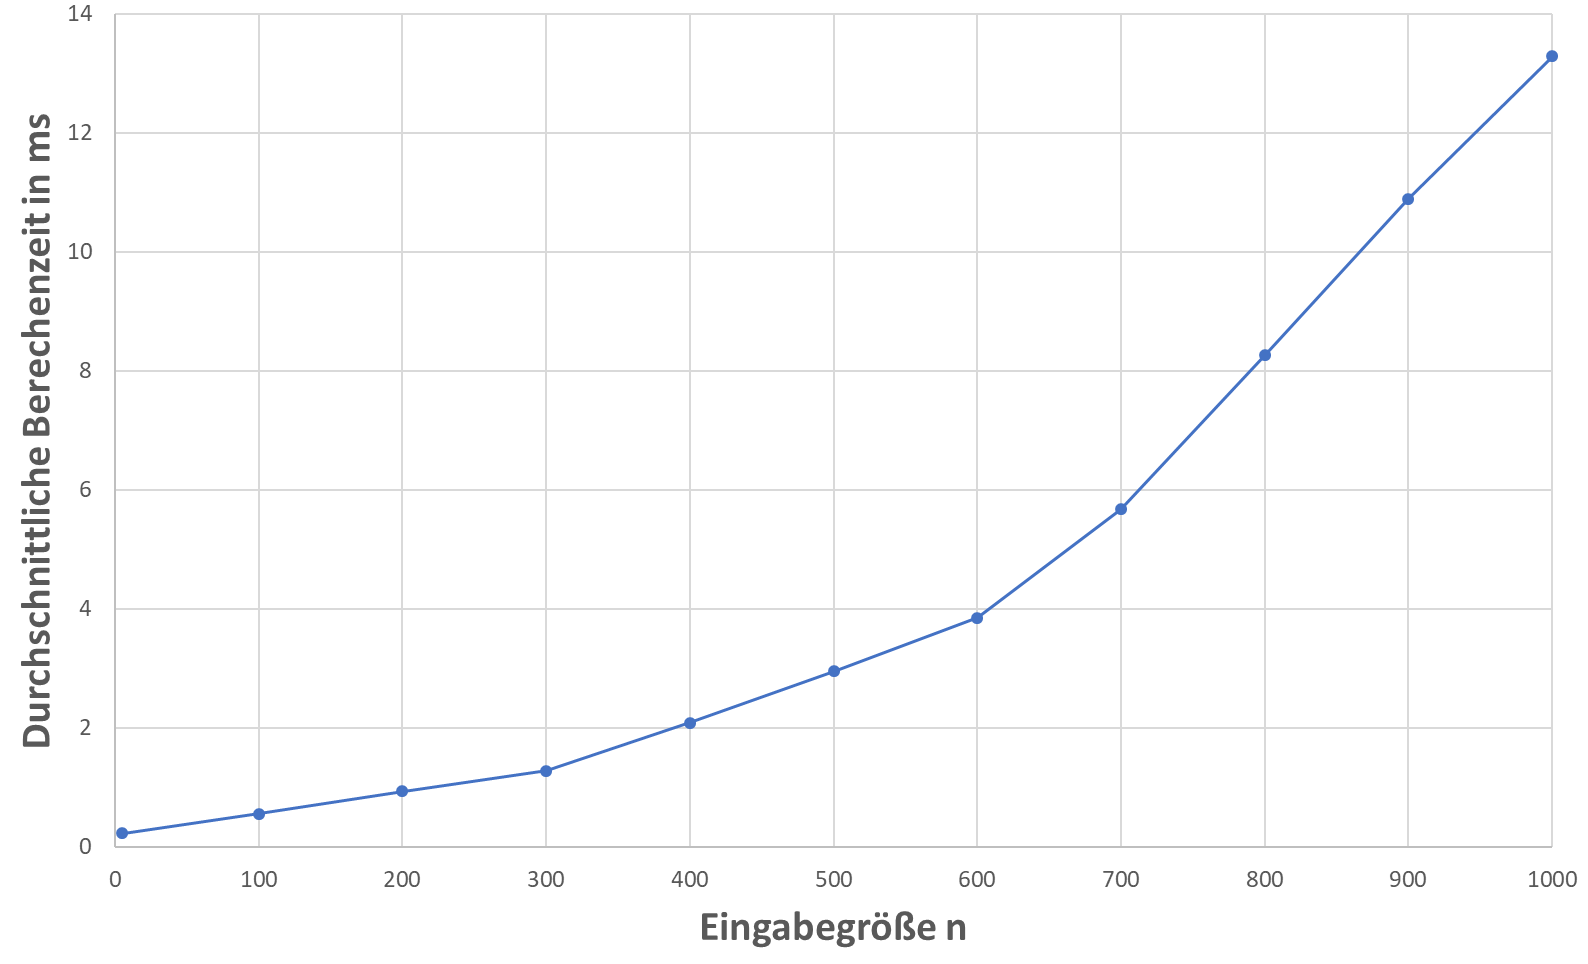
\includegraphics[scale=0.24]{../Verwendete/Exp1D_2.png}
\caption{blub}
\label{bla}
\end{figure}

\end{document}

%\draw[very thick] (-6,0) -- (6,0);
%\draw (0,0) -- (0,2); 